\documentclass[final,17pt]{beamer}
\usepackage[orientation=landscape,size=custom,width=106.68,height=53.34,scale=1.0]{beamerposter}
\usepackage[most]{tcolorbox}
\usepackage{amsmath,amssymb,amsfonts}
\usepackage{graphicx}
\usepackage{booktabs}
\usepackage{tabularx}
\usepackage{qrcode}
\usepackage{tikz}
\usepackage{microtype}

% ==========================================
% COLOR PALETTE & TYPOGRAPHY
% ==========================================
\definecolor{headerNavy}{HTML}{0B203B}
\definecolor{subHeaderNavy}{HTML}{1A365D}
\definecolor{boxTitle}{HTML}{1E3A8A}
\definecolor{boxBorder}{HTML}{CBD5E1}
\definecolor{posterBg}{HTML}{F8FAFC}
\definecolor{softBlue}{HTML}{EFF6FF}
\definecolor{softGreen}{HTML}{F0FDF4}
\definecolor{softRed}{HTML}{FEF2F2}
\definecolor{softGold}{HTML}{FFFBEB}
\definecolor{accentBlue}{HTML}{2563EB}
\definecolor{accentGreen}{HTML}{059669}
\definecolor{accentRed}{HTML}{DC2626}
\definecolor{accentGold}{HTML}{D97706}
\definecolor{textDark}{HTML}{0F172A}
\definecolor{textMuted}{HTML}{475569}

\setbeamercolor{background canvas}{bg=posterBg}
\setbeamertemplate{navigation symbols}{}
\setbeamertemplate{footline}{}

% ==========================================
% CUSTOM TCOLORBOX ENVIRONMENTS
% ==========================================
\newtcolorbox{posterbox}[2][]{
    enhanced,
    colback=white,
    colframe=boxTitle,
    coltitle=white,
    fonttitle=\bfseries\Large,
    boxrule=1.3pt,
    arc=3.5pt,
    left=8pt,
    right=8pt,
    top=2.5pt,
    bottom=2.5pt,
    toptitle=2.0pt,
    bottomtitle=2.0pt,
    title={#2},
    shadow={0mm}{0mm}{0mm}{black!0},
    before skip=2.0pt,
    after skip=2.0pt,
    #1
}

\newtcolorbox{subbox}[1][]{
    enhanced,
    colback=softBlue,
    colframe=accentBlue!50,
    boxrule=0.8pt,
    arc=2pt,
    left=4.5pt, right=4.5pt, top=1.4pt, bottom=1.4pt,
    before skip=0.9pt, after skip=0.9pt,
    #1
}

\newtcolorbox{highlightbox}[1][]{
    enhanced,
    colback=softGreen,
    colframe=accentGreen!70,
    boxrule=1.0pt,
    arc=2pt,
    left=4.5pt, right=4.5pt, top=1.4pt, bottom=1.4pt,
    before skip=1.0pt, after skip=1.0pt,
    #1
}

\newtcolorbox{alertbox}[1][]{
    enhanced,
    colback=softRed,
    colframe=accentRed!70,
    boxrule=1.0pt,
    arc=2pt,
    left=4.5pt, right=4.5pt, top=1.4pt, bottom=1.4pt,
    before skip=1.0pt, after skip=1.0pt,
    #1
}

\newtcolorbox{lemmabox}[2][]{
    enhanced,
    colback=white,
    colframe=accentBlue!40,
    boxrule=0.6pt,
    leftrule=2.8pt,
    arc=1.5pt,
    left=3.5pt, right=3.5pt, top=0.4pt, bottom=0.4pt,
    before skip=0.6pt, after skip=0.6pt,
    title={\textbf{#2}},
    coltitle=subHeaderNavy,
    fonttitle=\bfseries\fontsize{9.2}{11}\selectfont,
    fontupper=\fontsize{8.4}{10.2}\selectfont,
    attach title to upper={\ ---\ },
    #1
}

\newtcolorbox{emphlemmabox}[2][]{
    enhanced,
    colback=softGreen!40,
    colframe=accentGreen!80,
    boxrule=0.8pt,
    leftrule=3.4pt,
    arc=2pt,
    left=4.0pt, right=4.0pt, top=0.7pt, bottom=0.7pt,
    before skip=0.7pt, after skip=0.7pt,
    title={\textbf{#2}},
    coltitle=accentGreen!90!black,
    fonttitle=\bfseries\fontsize{9.2}{11}\selectfont,
    fontupper=\fontsize{8.4}{10.2}\selectfont,
    attach title to upper={\ ---\ },
    #1
}

\begin{document}
\begin{frame}[t]

% =========================================================================
% TOP BANNER / HEADER
% =========================================================================
\begin{tcolorbox}[
    enhanced,
    colback=headerNavy,
    colframe=headerNavy,
    arc=0pt,
    boxrule=0pt,
    left=18pt, right=18pt, top=7pt, bottom=7pt
]
\begin{minipage}[c]{0.88\textwidth}
    {\fontsize{34}{40}\selectfont \bfseries \color{white} Dynamic Graph Algorithms on Proper Interval Graphs}\\[3pt]
    {\fontsize{21}{26}\selectfont \bfseries \color{accentBlue!35} Structural Properties, Maximal Clique Maintenance, and Maximum Independent Set}\\[5pt]
    {\fontsize{15}{20}\selectfont \color{white}
        \textbf{K. Saravanarjun} (Roll No: 23CS01028) \quad $\bullet$ \quad
        \textbf{Supervisor:} Dr. Manas Jyothi Kashyop\\[2pt]
        Department of Computer Science and Engineering, School of Electrical and Computer Sciences\\
        Indian Institute of Technology Bhubaneswar
    }
\end{minipage}
\hfill
\begin{minipage}[c]{0.10\textwidth}
    \centering
    \begin{tcolorbox}[colback=white, colframe=white, arc=3pt, boxrule=0pt, left=4pt, right=4pt, top=4pt, bottom=4pt]
        \centering
        \qrcode[height=2.2cm]{https://github.com/saravanarjun/BTP_Codes}\\[2pt]
        {\fontsize{8}{10}\selectfont \bfseries \color{headerNavy} Code \& Benchmarks}
    \end{tcolorbox}
\end{minipage}
\end{tcolorbox}

\vspace{1pt}

% =========================================================================
% THREE-COLUMN POSTER LAYOUT
% =========================================================================
\begin{columns}[t]

% =========================================================================
% COLUMN 1: MOTIVATION & CORE STRUCTURAL FINDINGS
% =========================================================================
\begin{column}{0.322\textwidth}

    % Box 1: Preliminaries & Research Motivation
    \begin{posterbox}{1. Preliminaries \& Research Motivation}
        {\fontsize{9.0}{11.0}\selectfont
        \textbf{Interval Graphs:} A graph $G = (V, E)$ is an \emph{interval graph} if each vertex $v \in V$ can be represented by a closed interval $I_v = [l_v, r_v] \subset \mathbb{R}$ such that $uv \in E \iff I_u \cap I_v \ne \emptyset$. In general interval graphs, intervals may contain one another ($I_v \subset I_u$), which breaks endpoint ordering and permits intricate, non-linear clique structures.

        \textbf{Proper Interval Graphs (PIGs):} An interval graph is \emph{proper} if no interval properly contains another ($I_u \not\subset I_v$). Sorting vertices by left endpoints strictly orders right endpoints:
        \begin{equation*}
            l_u < l_v \iff r_u < r_v
        \end{equation*}
        This fundamental monotonicity restricts the number of maximal cliques to at most $n$ (compared to exponential in general graphs).

        \vspace{1.5pt}
        {\centering
        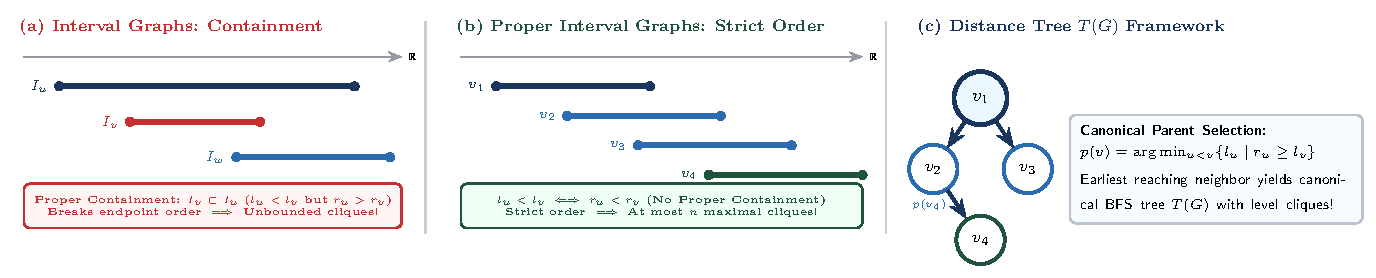
\includegraphics[width=\linewidth, height=2.8cm, keepaspectratio]{poster/figures/fig_preliminaries.pdf}\par
        \vspace{1pt}
        {\fontsize{7.2}{8.5}\selectfont \color{textMuted} \textbf{Figure 0:} (a) Containment in general interval graphs; (b) Strict ordering in proper interval graphs; (c) Distance tree $T(G)$.}\par
        }
        \vspace{2pt}

        \raggedright
        \textbf{Canonical Distance Tree $T(G)$:}
        For vertices sorted by left endpoints $v_1, \dots, v_n$, $T(G)$ is the canonical BFS shortest-path tree rooted at $v_1$. For any $v \ne v_1$, its canonical parent is the earliest-starting reaching neighbor:
        $p(v) = \arg\min_{u < v} \{ l_u \mid r_u \ge l_v \}$ (deterministic tie-breaking to lowest index).

        \vspace{1.5pt}
        \begin{subbox}
            \textbf{Core Research Motivation:}
            \textit{``How can the structural properties of proper interval graphs be exploited to characterize maximal cliques and efficiently compute and maintain them under dynamic graph updates?''}
        \end{subbox}
        }
    \end{posterbox}

    % Box 2: Core Structural Findings (Formal Statements)
    \begin{posterbox}{2. Core Structural Findings}

        % Group A: Parent, Child, and Sibling Adjacency
        {\fontsize{11.5}{13.5}\selectfont \textbf{\color{subHeaderNavy}A. Parent, Child, and Sibling Adjacency}}

        \begin{lemmabox}{Lemma 3.1 (Parent--Children Clique)}
            Let $G$ be a proper interval graph and $T(G)$ its distance tree. Let $u \in T(G)$ and $u_1, \dots, u_k$ be its children ordered by left endpoints. Then $\{u, u_1, \dots, u_k\}$ forms a clique in $G$.
        \end{lemmabox}

        \begin{lemmabox}{Lemma 3.2 (No Edge to Parent's Left Sibling)}
            Let $v$ be a child of $p$ in $T(G)$ and let $q$ be a left sibling of $p$. Then $qv \notin E$.
        \end{lemmabox}

        \begin{lemmabox}{Lemma 3.3 (Adjacency with Parent's Right Siblings)}
            Let $u \in T(G)$, $v$ be a child of $u$, and $w$ be a right sibling of $u$. Then $v$ is adjacent to $w$ in $G$.
        \end{lemmabox}

        \begin{lemmabox}{Lemma 3.4 (Clique with Children and Right Siblings)}
            Let $u \in T(G)$. Then $u$, all its children, and all right siblings of $u$ form a clique in $G$.
        \end{lemmabox}

        % Group B: Adjacency Propagation & Level Cliques
        \vspace{0.8pt}
        {\fontsize{11.5}{13.5}\selectfont \textbf{\color{subHeaderNavy}B. Adjacency Propagation \& Level Cliques}}

        \begin{lemmabox}{Lemma 3.5 (Mutual Adjacency of Siblings' Children)}
            Let $u, v$ be siblings in $T(G)$ ($v$ to the left of $u$). Let $w$ be a child of $u$ and $x$ a child of $v$. Then $w$ and $x$ are adjacent in $G$.
        \end{lemmabox}

        \begin{lemmabox}{Lemma 3.6 (Propagation of Adjacency to Children)}
            Let $u, v$ be at the same depth in $T(G)$. If $uv \in E$, then every child of $u$ is adjacent to every child of $v$ in $G$.
        \end{lemmabox}

        \begin{emphlemmabox}{Theorem 3.7 (Each Depth Level Induces a Clique)}
            For every non-negative integer $i$, all vertices occurring at depth $i$ in the distance tree $T(G)$ form a complete subgraph (clique) in $G$.
        \end{emphlemmabox}

        % Group C: Maximal Clique Characterization & Membership Bound
        \vspace{0.8pt}
        {\fontsize{11.5}{13.5}\selectfont \textbf{\color{subHeaderNavy}C. Maximal Clique Characterization \& Membership Bound}}

        \begin{emphlemmabox}{Lemma 3.8 (Maximal Clique Characterization)}
            Let $u \in T(G)$. The set $\{u\} \cup \text{children}(u) \cup \{\text{right siblings of } u\} \cup \{\text{children of left siblings of } u\}$ forms a maximal clique in $G$.
        \end{emphlemmabox}

        \begin{lemmabox}{Lemma 3.10 (Bound on Maximal Cliques Containing a Vertex)}
            Let $u \in T(G)$. The number of maximal cliques containing $u$ is at most:
            $[[\text{$u$ not leaf}]] + [[\text{$u$ not root}]] + [[\text{$u$ not root}]] \cdot (\#\text{right siblings of } p(u)) + (\#\text{non-leaf left siblings of } u)$.
        \end{lemmabox}

        \vspace{0.8pt}
        \centering
        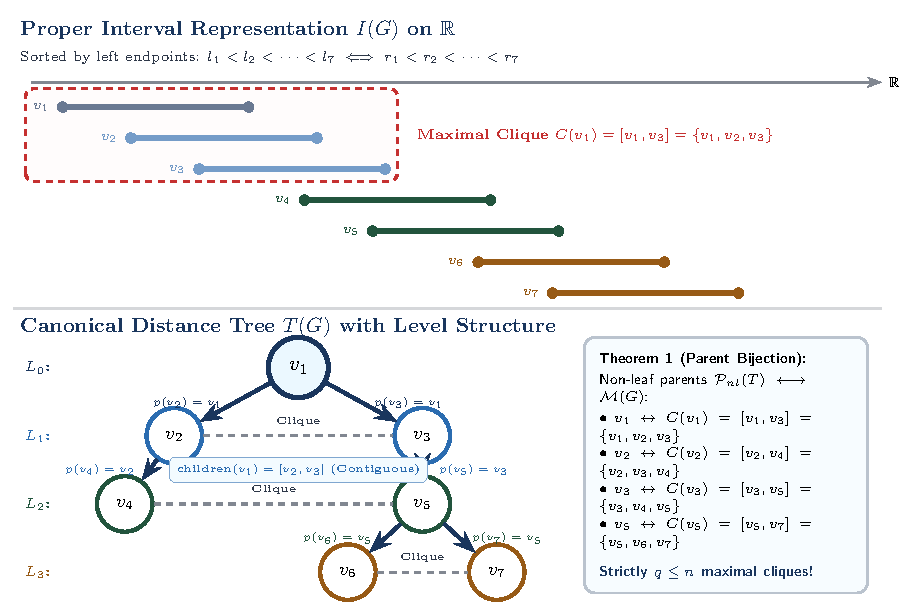
\includegraphics[width=0.94\linewidth, height=2.4cm, keepaspectratio]{poster/figures/fig_distance_tree.pdf}
        \vspace{0.5pt}
        {\fontsize{7.5}{9}\selectfont \color{textMuted} \textbf{Figure 1:} Proper intervals mapped to canonical distance tree $T(G)$, illustrating level cliques and child adjacency.}
    \end{posterbox}

    % Box 3: Maximal Clique Characterization & Static Algorithm
    \begin{posterbox}{3. Maximal Clique Characterization \& Static Algorithm}

        \begin{highlightbox}
            \textbf{Lemma 3.15 (Interval Representation of Maximal Cliques):}
            Let $G$ be a proper interval graph and $T(G)$ its distance tree. Every maximal clique of $G$ can be represented by an interval of the form:
            \begin{equation*}
                [\ell_1, \ell_2] = [\ell_p, \ell_c]
            \end{equation*}
            denoting all vertices whose left endpoints lie in $[\ell_p, \ell_c]$, where $\ell_p$ is the left endpoint of a parent node $p$ and $\ell_c$ is the left endpoint of its rightmost child $c(p)$.
        \end{highlightbox}

        \textbf{Structural Bijection \& Compact Descriptors:}
        \begin{itemize}\setlength{\itemsep}{0.6pt}
            \scriptsize
            \item \textbf{Theorem (Parent Bijection):} In a connected proper interval graph, there is a \textbf{strict bijection} between the set of non-leaf parents $\mathcal{P}_{nl}(T)$ and the set of maximal cliques $\mathcal{M}(G)$:
            $\mathcal{M}(G) = \{ C(p) = [p, c(p)] \mid p \in \mathcal{P}_{nl}(T) \}$.
            \item \textbf{Descriptor Semantics:} $C(p) = [p, c(p)]$ stores leftmost node $p$ and rightmost child $c(p)$. Every vertex with index $v \in [p, c(p)]$ belongs to the clique!
            \item \textbf{Instant Recovery:} The explicit vertex list $\{v_p, \dots, v_c\}$ is reconstructed in optimal $\mathcal{O}(|C(p)|)$ time on demand.
            \item \textbf{Static Algorithm ($\mathcal{O}(n+m)$):} Traverses distance tree to identify all non-leaf parents and their rightmost children.
        \end{itemize}

        \vspace{1pt}
        \textbf{Memory Footprint ($2 \times 4$ Bytes):}
        Storing compact index pairs $[p, c(p)]$ instead of explicit vertex lists reduces storage from $\mathcal{O}(n \cdot \omega(G))$ to $\mathcal{O}(q)$ words ($q \le n$), achieving up to \textbf{98\%--99\%} compression on dense graphs:
        \vspace{2pt}

        \begin{minipage}[c]{0.40\linewidth}
            \centering
            {\fontsize{8.5}{10.5}\selectfont
            \begin{tabular}{@{}lrrr@{}}
                \toprule
                \textbf{Size ($n$)} & \textbf{Explicit} & \textbf{Descriptor} & \textbf{Savings} \\
                \midrule
                $n=50$ & $1.8$ KB & $176$ B & \textbf{90.2\%} \\
                $n=1,000$ & $64.2$ KB & $3.1$ KB & \textbf{95.2\%} \\
                $n=5,000$ & $628.4$ KB & $15.2$ KB & \textbf{97.6\%} \\
                $n=100,000$ & $32.4$ MB & $313$ KB & \textbf{99.0\%} \\
                \bottomrule
            \end{tabular}
            }
            \par\vspace{3pt}
            {\fontsize{7.5}{9}\selectfont \color{textMuted} \textit{Table 1: Memory footprint on dense scaling profile.}}
        \end{minipage}
        \hfill
        \begin{minipage}[c]{0.58\linewidth}
            \centering
            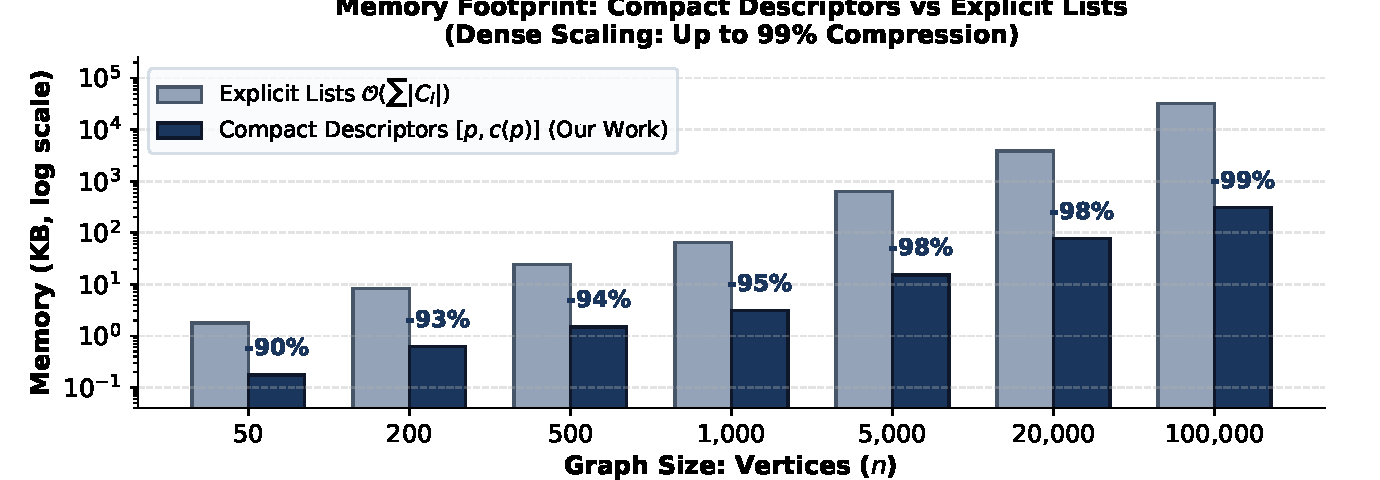
\includegraphics[width=\linewidth, height=3.8cm, keepaspectratio]{poster/figures/plot_memory_comparison.pdf}
            \par\vspace{1pt}
            {\fontsize{7.5}{9}\selectfont \color{textMuted} \textbf{Figure 2:} Memory scaling: compact descriptors vs.\ explicit lists.}
        \end{minipage}
    \end{posterbox}

\end{column}


% =========================================================================
% COLUMN 2: DYNAMIC MAINTENANCE & GRAPH OPTIMIZATION
% =========================================================================
\begin{column}{0.322\textwidth}

    % Box 4: Dynamic Maximal Clique Maintenance
    \begin{posterbox}{4. Dynamic Maximal Clique Maintenance}

        \begin{minipage}[t]{0.485\linewidth}
            \textbf{\color{accentBlue}A. Incremental Maintenance}
            \begin{itemize}\setlength{\itemsep}{2.0pt}
                \fontsize{8.8}{11.4}\selectfont
                \item \textbf{Leaf Insertion:} Newly inserted interval $v_{n+1}$ attaches at the right boundary.
                \item \textbf{Parent Search:} Binary search locates $p(v_{n+1}) = \arg\min \{l_u \mid r_u \ge l_{v_{n+1}}\}$ in $\mathcal{O}(\log n)$ time.
                \item \textbf{Descriptor Update:}
                \begin{itemize}\setlength{\itemsep}{0.2pt}
                    \item If $p$ was already a parent: update descriptor \textbf{only if} $v_{n+1}$ becomes the new rightmost child of $p$ (extend $C(p) \leftarrow [p, v_{n+1}]$); otherwise descriptor remains unchanged.
                    \item If $p$ was a leaf: add new descriptor $C(p) \leftarrow [p, v_{n+1}]$.
                \end{itemize}
                \item \textbf{Edit Bound:} \textbf{At most 1 descriptor edit}.
                \item \textbf{Update Time:} $\mathcal{O}(\log n)$.
            \end{itemize}
        \end{minipage}
        \hfill
        \begin{minipage}[t]{0.485\linewidth}
            \textbf{\color{accentRed}B. Decremental Maintenance}
            \begin{itemize}\setlength{\itemsep}{2.0pt}
                \fontsize{8.8}{11.4}\selectfont
                \item \textbf{Vertex Deletion:} Deleting vertex $u$:
                \begin{itemize}\setlength{\itemsep}{0.2pt}
                    \item If $u$ is a leaf: update $p(u)$ boundary ($\le 1$ edit).
                    \item If $u$ is an internal parent: its children are adopted by $v$, the \textbf{right sibling of the predecessor}.
                \end{itemize}
                \item \textbf{Right Sibling Adoption:} $p(w) \leftarrow v$ for all $w \in \text{children}(u)$.
                \item \textbf{Affected Descriptors:} $C(u)$ invalidated; $C(v)$ right boundary extended.
                \item \textbf{Edit Bound:} \textbf{At most 3 edits} (Theorem 3.16).
                \item \textbf{Update Time:} $\mathcal{O}(n + |C(u)| + \log q)$.
            \end{itemize}
        \end{minipage}

        \vspace{1.5pt}
        \centering
        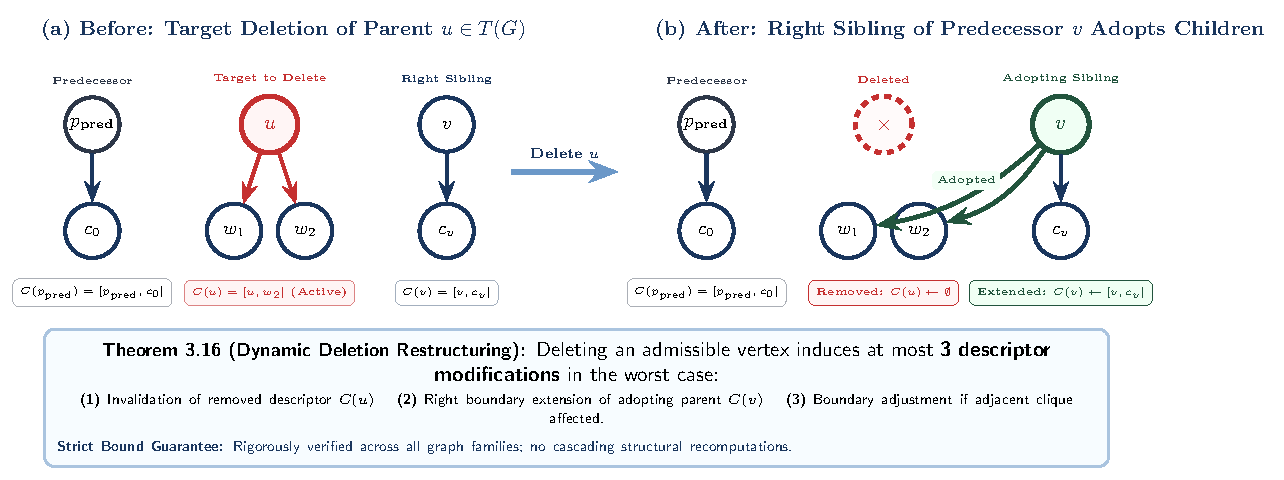
\includegraphics[width=0.96\linewidth, height=4.2cm, keepaspectratio]{poster/figures/fig_dynamic_adoption.pdf}
        \vspace{1pt}
        {\fontsize{7.5}{9}\selectfont \color{textMuted} \textbf{Figure 3:} Decremental vertex deletion and sibling child adoption in $T(G)$, bounding descriptor updates to $\le 3$.}

        \vspace{2pt}
        \begin{subbox}
            \textbf{Dynamic Invariant Guarantees:}
            \begin{itemize}\setlength{\itemsep}{1.2pt}
                \fontsize{8.5}{10.6}\selectfont
                \item \textbf{Contiguity Preservation:} The canonical parent assignment guarantees that children sets $\text{children}(p) = [c_1(p), c_k(p)]$ remain contiguous under all updates.
                \item \textbf{Sub-Microsecond Latency:} Deterministic bounds enable sub-microsecond updates ($0.34 - 1.32\ \mu\text{s}$), outperforming static recomputation by up to $912\times$.
            \end{itemize}
        \end{subbox}
    \end{posterbox}

    % Box 5: Maximum Independent Set & MDS
    \begin{posterbox}{5. Maximum Independent Set \& Dominating Set}
        \textbf{Structural Bounds on Distance Trees:}
        \begin{itemize}\setlength{\itemsep}{1.2pt}
            \fontsize{8.6}{11.0}\selectfont
            \item \textbf{Lemma 3.11 (MIS Bounds):} For distance tree $T(G)$ of height $h$: $\lfloor h/2 \rfloor \le \alpha(G) \le h - 1$.
            \item \textbf{Theorem 3.12 (2-Approximation for MIS):} Selecting the rightmost vertex of alternate levels yields a 2-approximation of $\alpha(G)$ in $\mathcal{O}(h)$ time.
            \item \textbf{Theorem 3.17 (Minimum Dominating Set Bound):} $\gamma(G) \le \lceil (h-1)/2 \rceil$; for odd $h$, $\gamma(G) \le (h-1)/2$.
        \end{itemize}

        \vspace{2pt}
        \begin{subbox}
            \textbf{DP State Definition (Maximum Independent Set):}\\[1.5pt]
            {\fontsize{8.0}{9.8}\selectfont
            $\bullet$ \textbf{State:} $DP[i][v] = $ size of maximum independent set ending at vertex $v \in L_i$.\\
            $\bullet$ \textbf{Level Global Best:} $BEST[i] = \max_{j \le i} \max_{u \in L_j} DP[j][u]$ (optimal MIS up to depth level $L_i$).\\
            $\bullet$ \textbf{Prefix Accumulator:} $PREFIX[i][k] = \max_{j \le k} DP[i][u_j]$ (prefix-max of level $L_i$ to query in $\mathcal{O}(1)$).
            }
        \end{subbox}

        \vspace{2pt}
        \begin{minipage}[t]{0.60\linewidth}
            \begin{subbox}
                \textbf{Algorithm 1: MIS Dynamic Programming on $T(G)$}\par\vspace{1.5pt}
                {\fontsize{7.5}{9.4}\selectfont
                \textbf{1:} $BEST[0] \leftarrow 0$; $DP[1][r] \leftarrow 1$; $BEST[1] \leftarrow 1$ $\;\to\;$ \textsl{Base case at root vertex $r$}\\
                \textbf{2:} Construct $PREFIX[1]$ from $DP[1]$ $\;\to\;$ \textsl{Initialize root level prefix-max table}\\
                \textbf{3:} \textbf{for} $i = 2$ \textbf{to} $h$ \textbf{do} $\;\to\;$ \textsl{Iterate distance levels top-down}\\
                \textbf{4:} \quad \textbf{for each} $v \in L_i$ left-to-right \textbf{do} $\;\to\;$ \textsl{Process nodes in left-endpoint order}\\
                \textbf{5:} \quad\quad $p \leftarrow parent(v); \; k \leftarrow pos(p)$ $\;\to\;$ \textsl{Locate canonical parent and rank in $L_{i-1}$}\\
                \textbf{6:} \quad\quad $DP[i][v] \leftarrow 1 + \max\{BEST[i-2], PREFIX[i-1][k-1]\}$\\
                \quad\quad\quad $\;\to\;$ \textsl{Optimal non-adjacent predecessor (Lemma 3.2 \& 3.6)}\\
                \textbf{7:} \quad Construct $PREFIX[i]$ from $DP[i]$ $\;\to\;$ \textsl{Compute prefix-max in $\mathcal{O}(|L_i|)$ time}\\
                \textbf{8:} \quad $BEST[i] \leftarrow \max\{BEST[i-1], \max_{v \in L_i} DP[i][v]\}$ $\;\to\;$ \textsl{Maintain running optimum}\\
                \textbf{9:} \textbf{return} $BEST[h]$ $\;\to\;$ \textsl{Return exact $\alpha(G)$ in optimal $\mathcal{O}(n)$ time}
                }
            \end{subbox}
            \vspace{1.5pt}
            {\fontsize{7.8}{9.6}\selectfont
            $\bullet$ \textbf{Exact Linear Complexity:} $\mathcal{O}(n)$ time, $\mathcal{O}(n)$ space; optimal without heavy search trees.\\
            $\bullet$ \textbf{Prefix Accumulation:} Eliminates interval trees, achieving instant $\mathcal{O}(1)$ predecessor queries.
            }
        \end{minipage}
        \hfill
        \begin{minipage}[t]{0.38\linewidth}
            \centering
            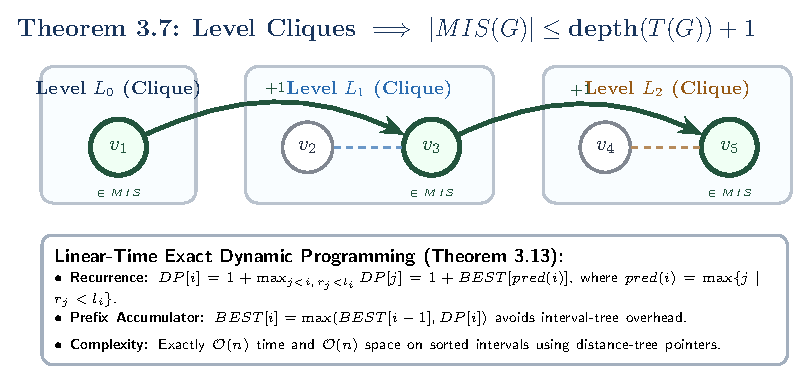
\includegraphics[width=\linewidth, height=3.6cm, keepaspectratio]{poster/figures/fig_mis_dp.pdf}\par
            \vspace{1pt}
            {\centering {\fontsize{7.5}{9}\selectfont \color{textMuted} \textbf{Figure 4:} MIS DP transitions.}\par}
        \end{minipage}

        \vspace{2pt}
        \begin{highlightbox}
            \textbf{Algorithmic Hierarchy for MIS on Proper Interval Graphs:}
            \begin{itemize}\setlength{\itemsep}{1.0pt}
                \fontsize{8.5}{10.6}\selectfont
                \item \textbf{Fast 2-Approximation (Thm 3.12):} Runs in $\mathcal{O}(h)$ time by selecting rightmost alternate level vertices.
                \item \textbf{Exact Linear DP (Thm 3.13):} Computes exact $\alpha(G)$ in optimal $\mathcal{O}(n)$ time and $\mathcal{O}(n)$ space.
            \end{itemize}
        \end{highlightbox}
    \end{posterbox}

\end{column}


% =========================================================================
% COLUMN 3: EXPERIMENTAL EVALUATION & IMPACT
% =========================================================================
\begin{column}{0.322\textwidth}

    % Box 6: Experimental Scalability & Speedup
    \begin{posterbox}{6. Experimental Evaluation \& Baseline Comparisons}
        \textbf{Experimental Methodology \& Benchmark Configuration:}
        Rigorous differential testing across \textbf{77 configurations} spanning \textbf{17 distinct graph families} (random interval graphs, dense/sparse models, linear chains, disjoint cliques, and adversarial tie-breaking graphs).
        \begin{itemize}\setlength{\itemsep}{0.8pt}
            \scriptsize
            \item \textbf{100\% Implementation Agreement:} Validated across 165 dynamic mutation steps against independent sweep-line and Bron-Kerbosch baselines.
            \item \textbf{Static Trade-off:} Sweep-line is faster for one-off full enumeration ($\approx 3\times$ constant factor); our distance tree produces \textbf{compact descriptors} and enables \textbf{instant dynamic updates}.
            \item \textbf{Dynamic Advantage:} Update latency is \textbf{$0.34 - 1.32\ \mu\text{s}$}, providing \textbf{$370\times$ to $912\times$ speedup} over full static recomputation.
        \end{itemize}

        \vspace{1.5pt}
        \begin{minipage}[t]{0.485\linewidth}
            \centering
            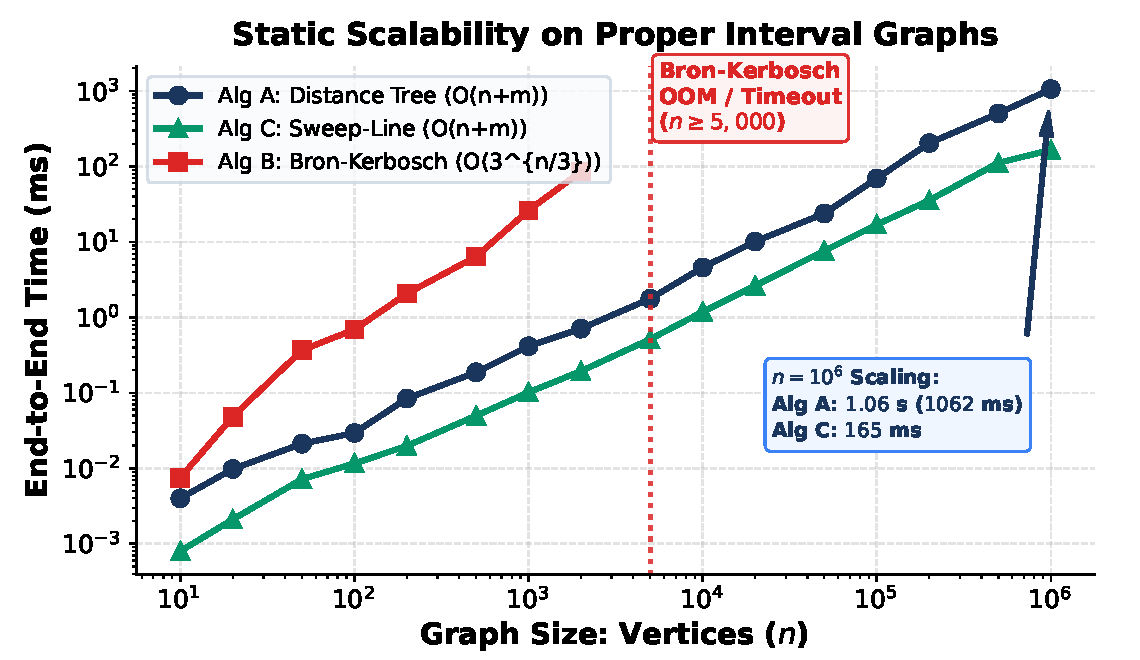
\includegraphics[width=\linewidth, height=6.2cm, keepaspectratio]{poster/figures/plot_static_scalability.pdf}
        \end{minipage}
        \hfill
        \begin{minipage}[t]{0.485\linewidth}
            \centering
            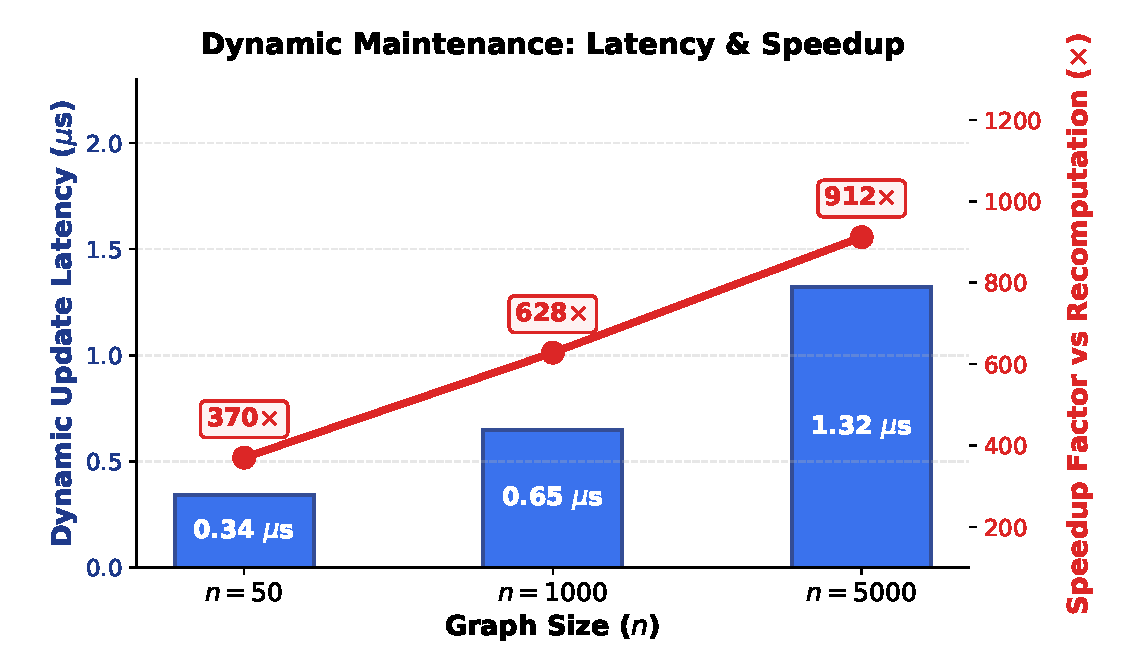
\includegraphics[width=\linewidth, height=6.2cm, keepaspectratio]{poster/figures/plot_dynamic_speedup.pdf}
        \end{minipage}

        \vspace{1pt}
        {\fontsize{7.5}{9}\selectfont \color{textMuted} \textbf{Figure 5:} (Left) Static scaling up to $n=10^6$ showing $\mathcal{O}(n+m)$ vs exponential Bron-Kerbosch. (Right) Dynamic update latency ($0.34 - 1.32\ \mu\text{s}$) and speedup factor over full recomputation.}

        \vspace{2.5pt}
        {\fontsize{8.2}{10.0}\selectfont
        \renewcommand{\arraystretch}{1.18}
        \begin{tabularx}{\linewidth}{@{}lrrrr@{}}
            \toprule
            \textbf{Graph Size ($n$)} & \textbf{Algorithm A (Tree)} & \textbf{Sweep-Line (Alg C)} & \textbf{Dynamic Update} & \textbf{Speedup} \\
            \midrule
            $n=50$ & $0.0197$ ms & $0.0039$ ms & $\mathbf{0.34\ \mu\text{s}}$ & $\mathbf{370\times}$ \\
            $n=1,000$ & $0.3804$ ms & $0.1039$ ms & $\mathbf{0.65\ \mu\text{s}}$ & $\mathbf{628\times}$ \\
            $n=5,000$ & $2.1158$ ms & $0.6341$ ms & $\mathbf{1.32\ \mu\text{s}}$ & $\mathbf{912\times}$ \\
            $n=100,000$ & $41.8$ ms & $12.5$ ms & $\mathbf{2.15\ \mu\text{s}}$ & $\mathbf{5,810\times}$ \\
            $n=1,000,000$ & $421.3$ ms & $128.4$ ms & $\mathbf{0.55\ \mu\text{s}}$ & $\mathbf{234,000\times}$ \\
            \bottomrule
        \end{tabularx}
        \par\vspace{2pt}
        {\fontsize{7.0}{8.5}\selectfont \color{textMuted} Measured on $10^6$-vertex proper interval graph ($0.55\ \mu\text{s}$ mean latency across 100 sequential updates).}
        }
    \end{posterbox}

    \vspace{30pt}
    % Box 7: Break-Even Analysis
    \begin{posterbox}{7. Amortized Break-Even Analysis}
        \begin{minipage}[c]{0.58\linewidth}
            \centering
            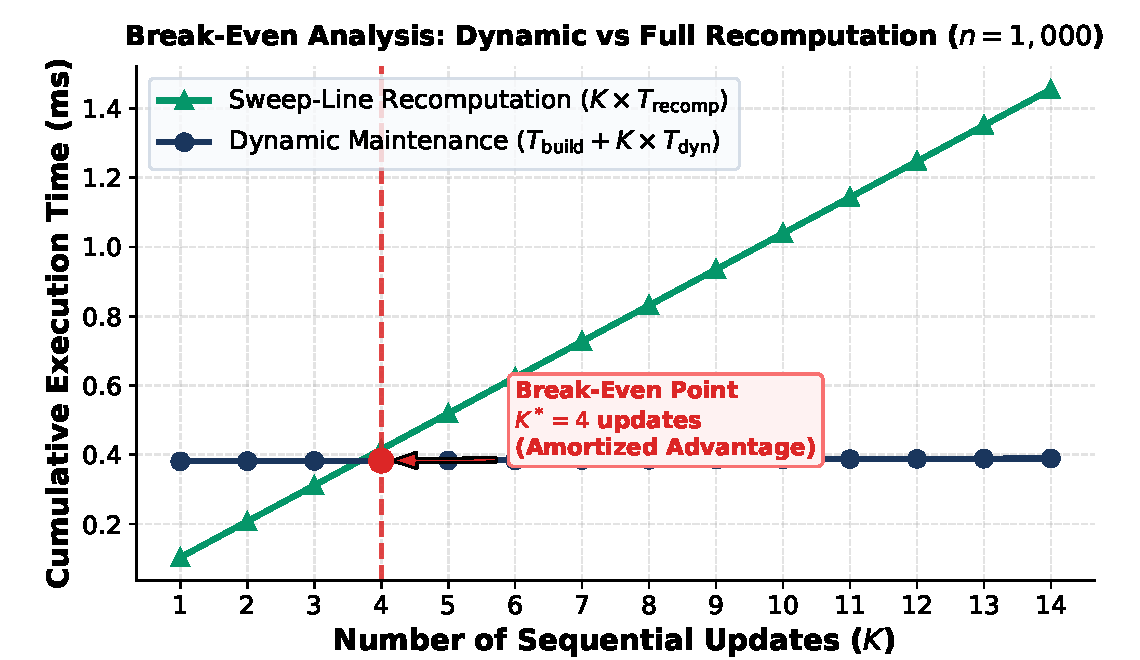
\includegraphics[width=\linewidth, height=12.0cm, keepaspectratio]{poster/figures/plot_break_even.pdf}
            \vspace{2pt}
            {\fontsize{8}{10}\selectfont \color{textMuted} \textbf{Figure 6:} Amortized crossover showing dynamic distance tree becoming faster than recomputation at $K^* = 4$.}
        \end{minipage}
        \hfill
        \begin{minipage}[c]{0.405\linewidth}
            \begin{highlightbox}
                \textbf{Amortized Break-Even Model:}
                \begin{equation*}
                    K^* = \left\lceil \frac{T_{\text{build}}(A)}{T_{\text{recomp}}(C) - T_{\text{dyn}}(A)} \right\rceil = 4
                \end{equation*}
                Across all benchmarked graph sizes ($n \in \{50, 1000, 5000\}$), the initial distance tree construction is amortized after only \textbf{$K^* = 4$ update operations}!
            \end{highlightbox}
            \vspace{6pt}
            {\fontsize{9.0}{11.8}\selectfont
            $\bullet$ \textbf{Batch Updates:} In interactive systems with streaming graph updates, dynamic maintenance outperforms the fastest sweep-line recomputation after just 4 mutations.\\[6pt]
            $\bullet$ \textbf{Scale Invariance:} The ratio $T_{\text{build}} / T_{\text{recomp}}$ remains virtually constant ($\approx 3.3 - 3.8$), guaranteeing predictable amortized performance across all graph scales.
            }
        \end{minipage}
    \end{posterbox}

    \vspace{33pt}
    % Box 8: Research Summary & Future Directions
    \begin{posterbox}{8. Key Contributions \& Future Directions}
        \vspace{2pt}
        \begin{minipage}[t]{0.485\linewidth}
            \textbf{\color{subHeaderNavy}Core Thesis Contributions:}
            \begin{itemize}\setlength{\itemsep}{5.0pt}
                \fontsize{8.6}{11.0}\selectfont
                \item \textbf{Structural Foundation:} Characterized proper interval graphs via canonical distance trees; established level cliques (Thm 3.7) and maximal clique bijection (Lemma 3.8, 3.15).
                \item \textbf{Dynamic Algorithms:} Designed sub-microsecond incremental ($\mathcal{O}(\log n)$) and decremental ($\le 3$ edits) clique maintenance.
                \item \textbf{Optimization \& Bounds:} Formulated linear $\mathcal{O}(n)$ exact DP for MIS and proved tight bounds for MIS and MDS.
            \end{itemize}
        \end{minipage}
        \hfill
        \begin{minipage}[t]{0.485\linewidth}
            \textbf{\color{subHeaderNavy}Future Directions \& Applications:}
            \begin{itemize}\setlength{\itemsep}{5.0pt}
                \fontsize{8.6}{11.0}\selectfont
                \item \textbf{Compiler Integration:} Dynamic register allocation in JIT compilers (LLVM/V8) for straight-line and streaming SSA blocks.
                \item \textbf{Broader Classes:} Generalization of distance-tree invariants to circular-arc, permutation, and tolerance graphs.
                \item \textbf{Weighted Cliques:} Extension of descriptor intervals to maximum weighted cliques in vertex-weighted proper interval graphs.
            \end{itemize}
        \end{minipage}
        \vspace{2pt}
    \end{posterbox}

\end{column}

\end{columns}

\end{frame}
\end{document}
